\documentclass[ijoc]{informs3}
\OneAndAHalfSpacedXI
\usepackage{natbib}
 \bibpunct[, ]{(}{)}{,}{a}{}{,}%
 \def\bibfont{\small}%
 \def\bibsep{\smallskipamount}%
 \def\bibhang{24pt}%
 \def\newblock{\ }%
 \def\BIBand{and}%
\TheoremsNumberedThrough
\ECRepeatTheorems
\EquationsNumberedThrough
\usepackage{amsmath,amssymb,booktabs,graphicx,enumitem,algorithm,algpseudocode}
\usepackage[capitalize]{cleveref}
\newcommand{\R}{\mathbb{R}}
\newcommand{\Om}{\mathcal{O}(m)}

\begin{document}
\RUNAUTHOR{Livne}
\RUNTITLE{Near-linear bilevel congestion network design}
\TITLE{A Near-Linear-Time Solver for Bilevel Congestion Network Design
via Directed Nonlinear Laplacian Flow}
\ARTICLEAUTHORS{%
\AUTHOR{Oren E. Livne}
\AFF{Pine Birch Analytics, Churchville, PA, \EMAIL{oren.livne@gmail.com}}
}
\ABSTRACT{
Bilevel traffic network design---optimizing link tolls or capacities over a lower-level user
equilibrium---is the workhorse formulation of congestion pricing, capacity planning, and origin--destination
calibration. It is nonconvex and \emph{NP}-hard, and every practical method solves it by an outer optimization
whose each step requires a lower-level equilibrium solve together with an equilibrium sensitivity. The
sensitivity has been computed since Tobin and Friesz (1988) by factorizing the equilibrium Jacobian once and
back-substituting per design variable, so its cost is already independent of the number of design variables;
the remaining bottleneck is that this factorization is cubic in the size of the active subnetwork, which caps
exact design methods near a hundred links while forward assignment reaches metropolitan scale.
We remove that bottleneck. We show that the \emph{directed} user equilibrium with separable costs is a
source-form nonlinear Laplacian flow $B\rho(B^\top\phi-\tau)=d$ whose Newton Jacobian, despite the
one-sided (rectified) edge law, remains a \emph{symmetric weighted graph Laplacian on the active subgraph}.
Consequently the whole solve---forward equilibrium \emph{and} adjoint design gradient---reduces to a short
sequence of near-linear Laplacian solves. The one obstacle, that the rectified dead zone makes the Jacobian
ill-conditioned and its active set change during a solve, is handled by a smoothing homotopy in a dead-zone
width $\delta$ that keeps the linearized system uniformly well conditioned, followed by a single exact-law
polish. On the Sioux Falls network the solver matches Frank--Wolfe to $10^{-11}$, the adjoint gradient matches
central finite differences to within finite-difference error, and projected-gradient toll design reduces total
system travel time monotonically to the exact (marginal-cost) optimum. The number of algebraic-multigrid setups
per equilibrium solve is bounded independently of the graph size, and the wall-clock scales near-linearly in the
edge count while a direct factorization scales superlinearly, so on large \emph{irregular} congestion networks
(scale-free communication and overlay topologies) the near-linear solver overtakes the direct factorization at a
crossover; the design optimization inherits this near-linear per-step cost. Road networks, being near-planar, are
the regime where a direct nested-dissection factorization is already near-optimal and the near-linear solver does
\emph{not} win; the advantage is on the poorly-separable networks that model selfish routing in communication
systems. We further extend the framework to the \emph{multicommodity} logit stochastic
user equilibrium, where the Newton system is a coupled block-Laplacian that a distribution-matrix block
preconditioner solves in a handful of iterations, and the design adjoint again returns the gradient for all
tolls in one solve; on the Sioux Falls and Anaheim road networks with their published origin--destination
matrices, destination-bundled design cuts total system travel time by $7.7$--$13.1\%$ with a bounded
inner-iteration count. Code is available at \url{https://github.com/orenlivne/dnlf}.
}

\KEYWORDS{network design; traffic assignment; user equilibrium; bilevel optimization; nonlinear Laplacian
flow; algebraic multigrid; adjoint sensitivity; congestion pricing}

\maketitle

\section{Introduction}\label{sec:intro}
Given a road network with $m$ directed links and travel-time (latency) functions $t_a(f_a)$ that increase with
flow, the \emph{lower-level} user equilibrium (UE) assigns origin--destination demand so that no traveler can
lower their experienced cost by switching route (Wardrop's principle). The \emph{upper-level} \emph{network
design problem} chooses $k$ design variables $\tau$---link tolls in congestion pricing, capacity expansions in
the continuous network design problem (CNDP), or a demand table in OD calibration---to minimize a system
objective $F$, most commonly total system travel time (TSTT), subject to the induced equilibrium:
\begin{equation}\label{eq:bilevel}
\min_{\tau\in\mathcal{T}}\; F\big(f^\star(\tau)\big)
\qquad\text{s.t.}\qquad f^\star(\tau)\ \text{solves the UE at design }\tau .
\end{equation}
This bilevel program is the standard model for congestion pricing, capacity planning, and demand estimation.
It is nonconvex, nondifferentiable, and \emph{NP}-hard even with affine latencies~\citep{gairing2017}; second-best
tolling is \emph{NP}-hard as well~\citep{hoefer2008}. Practical methods therefore seek a local (KKT) stationary
point, and essentially all of them---sensitivity-analysis-based (SAB) descent~\citep{tobinfriesz1988,jp2007,chiou2005},
mathematical programs with equilibrium constraints, and metaheuristics---run an \emph{outer}
loop where each iteration solves the lower-level equilibrium and then a sensitivity (equilibrium derivative).

\subsection{Computational cost, and where it lives}
The design gradient itself is cheap in the number of design variables: since \citet{tobinfriesz1988}, $\nabla_\tau F$ is obtained by factorizing the equilibrium Jacobian \emph{once}
and back-substituting one right-hand side per design variable, so its cost is independent of $k$ (an adjoint /
implicit-function computation~\citep{jp2007,amos2017,blondel2022}). The bottleneck is that this
factorization and the lower-level solve that precedes it are direct sparse factorizations whose cost is cubic in the active-path/subnetwork size, or a slowly converging Frank--Wolfe assignment. This
is why exact design methods in the literature stall near Sioux Falls scale ($76$ links) while origin-based
forward assignment routinely reaches $40,000$--$75,000$ links~\citep{bargera2002,dial2006}. The gap
between forward and design scalability is one to two orders of magnitude, and is purely a linear-algebra gap.

\subsection{Contribution}
We close that gap by replacing the superlinear inner factorization with a near-linear one for both the forward
equilibrium and the adjoint, without compromising accuracy. Our contributions are:
\begin{enumerate}[leftmargin=*]
\item \textbf{A Laplacian formulation of the directed equilibrium (\cref{sec:formulation}).} We write the
separable directed UE as a source-form nonlinear Laplacian flow $B\rho(B^\top\phi-\tau)=d$ with a one-sided
(rectified) edge law, and show that the Newton Jacobian is a \emph{symmetric} graph Laplacian on the
active subgraph (\cref{prop:laplacian}). Orientation and one-sidedness do not break the Laplacian; they only
determine which arcs are active. Hence the near-linear Laplacian toolbox applies.
\item \textbf{A near-linear equilibrium solver robust to the dead zone (\cref{sec:solver}).} The rectified law
is nonsmooth: a link carries flow only once its potential drop exceeds the free-flow cost $t^0_a$, so the active
set---and the conditioning of the Jacobian---changes during a solve, defeating a naively frozen multigrid
hierarchy. We introduce a \emph{smoothing homotopy}: a softplus dead-zone width $\delta$ that keeps the
conductance strictly positive and the linearized system uniformly well conditioned, continued from a smooth
problem to the exact law, with one algebraic-multigrid (AMG) setup per $\delta$-level and a final exact-law
polish. The number of setups is bounded independently of graph size.
\item \textbf{A near-linear adjoint and design loop (\cref{sec:design}).} The design gradient is one additional
Laplacian solve with the same operator; projected-gradient descent on it drives TSTT monotonically to the
stationary point.
\item \textbf{Validation (\cref{sec:results}).} On Sioux Falls the solver matches Frank--Wolfe to $10^{-11}$;
the adjoint matches finite differences to finite-difference accuracy; toll design reaches the exact
marginal-cost optimum. Setups per solve are bounded in graph size and the wall-clock scales near-linearly in
$m$, so design inherits the near-linear inner cost.
\end{enumerate}
\subsection{Scope: Irregular Networks}
The lower-level equilibrium \cref{eq:nlf} is the Wardrop equilibrium of a nonlinear congestion
game~\citep{rosenthal1973,roughgarden2002}, and the design problem \cref{eq:bilevel} is the optimal-tolling /
Stackelberg problem of reducing the price of anarchy~\citep{swamy2012,korilis1997}. This model describes selfish
routing not only in road traffic but in communication and overlay networks such as multipath and elastic-traffic
routing games in the Internet, data-center fabrics, and peer-to-peer overlays~\citep{orda1993,larroca2013}. The
distinction matters for scalability: road networks are near-planar, where a direct nested-dissection
factorization of the equilibrium Jacobian is already near-optimal. Communication and overlay topologies, by contrast, are large and \emph{poorly separable} (scale-free
degree, no planar embedding), so a direct factorization fills in superlinearly---exactly the regime in which a
near-linear Laplacian solver wins. Our scaling study is therefore on irregular networks; for the time we focus on establishing the near-linear advantage only here. The most literal instance is selfish
\emph{overlay} routing, where end hosts genuinely choose paths~\citep{qiu2003}, on Internet AS- and router-level
graphs that are provably scale-free~\citep{faloutsos1999}. Production traffic engineering
optimizes operator-set link weights or bandwidth allocations by linear programming and local
search~\citep{fortz2000}, not by pricing a selfish equilibrium, and packet-level congestion control is a distinct
(utility-maximization) equilibrium. Our contribution is thus methodological, a scalable solver for the well-established
equilibrium/design model on standard large irregular topologies, complementing rather than replacing
operator tools.

The construction reuses the nonlinear Laplacian flow (NLF) solver~\citep{nlf} and its near-linear inner engine,
Lean Algebraic Multigrid (LAMG+)$+$~\citep{lamgplus} (approximate Cholesky~\citep{kyngsachdeva2016} is interchangeable and has a smaller hidden constant but is less robust here). We treat both the single-commodity
directed equilibrium (\crefrange{sec:formulation}{sec:results}) and its multicommodity logit stochastic-user-
equilibrium extension (\cref{sec:mc}), where a distribution-matrix block preconditioner keeps the inner solve
to a handful of iterations. Active-set deflation that would support a single hierarchy valid across all design steps (reducing setups from $\mathcal{O}(1)$-per-solve to $\mathcal{O}(1)$
total) is an open problem (\cref{sec:conclusion}).

\section{The directed equilibrium is a nonlinear Laplacian flow}\label{sec:formulation}
Let $B\in\R^{n\times m}$ be the node--arc incidence matrix of the directed network, $B_{\cdot a}=e_{h(a)}-e_{t(a)}$
for arc $a$ from tail $t(a)$ to head $h(a)$. Separable BPR latencies are $t_a(f)=t^0_a\big(1+\beta_a(f/c_a)^{p_a}\big)$
for $f\ge 0$. With node potentials $\phi$ (multipliers of conservation $Bf=d$) and toll $\tau_a\ge0$, the
Karush--Kuhn--Tucker conditions of the Beckmann program $\min_{f\ge0,\,Bf=d}\sum_a\int_0^{f_a}(t_a(x)+\tau_a)\,dx$
give the \emph{rectified} edge law
\begin{equation}\label{eq:rho}
f_a=\rho_a(g_a-\tau_a),\qquad g_a:=(B^\top\phi)_a=\phi_{t(a)}-\phi_{h(a)},\qquad
\rho_a(u)=\begin{cases} t_a^{-1}(u), & u> t^0_a,\\[1pt] 0, & u\le t^0_a,\end{cases}
\end{equation}
so that conservation becomes the source-form nonlinear Laplacian flow
\begin{equation}\label{eq:nlf}
B\,\rho(B^\top\phi-\tau)=d .
\end{equation}
The law is monotone but \emph{one-sided}: unlike the odd law of the undirected Beckmann relaxation, $\rho_a$ has a
dead zone $u\le t^0_a$ in which the arc is unused. This dead zone is exactly what distinguishes the directed
equilibrium from its undirected relaxation.

\begin{proposition}\label{prop:laplacian}
For separable costs the Newton Jacobian of \cref{eq:nlf} is a symmetric, positive semidefinite weighted graph
Laplacian supported on the active arcs. Explicitly, with $\rho'_a\ge0$,
\[
J=B\,\mathrm{diag}(\rho')\,B^\top=\sum_{a}\rho'_a\,(e_{t(a)}-e_{h(a)})(e_{t(a)}-e_{h(a)})^\top ,
\quad \rho'_a=\tfrac{1}{t'_a(f_a)}>0 \text{ (active)},\ \rho'_a=0 \text{ (else)}.
\]
\end{proposition}
\begin{proof}{\it Proof.}
Differentiating \cref{eq:nlf} in $\phi$ gives $J=B\,\mathrm{diag}(\rho'(B^\top\phi-\tau))\,B^\top$. The rank-one
term $(e_{t(a)}-e_{h(a)})(e_{t(a)}-e_{h(a)})^\top$ is independent of the arc's orientation, and $\rho'_a\ge0$
because $t_a$ is increasing; hence $J\succeq0$ is a weighted Laplacian, with weight $\rho'_a=0$ precisely on
inactive (dead-zone) arcs. \qed
\end{proof}

\Cref{prop:laplacian} is the structural fact this paper rests on: directedness enters only through \emph{which}
arcs are active (a routing boundary), not through the type of the linear operator. Every linearized system is a
graph Laplacian, which can be solved fast. This is complete for the single-commodity
equilibrium (a general balanced demand, possibly multi-source/multi-sink). The multicommodity case
($f_a=\sum_k f_a^k$ with a cost of the total flow) yields a coupled \emph{block} system---per-commodity
Laplacians with a rank-one commodity coupling per arc---which a distribution-matrix block preconditioner still
solves in a handful of iterations; we develop this in \cref{sec:mc} (\cref{prop:mc}).

\section{A near-linear equilibrium solver}\label{sec:solver}
We solve \cref{eq:nlf} by damped chord-Newton on the frozen-linearization Jacobian $J$, delegating each
linearized solve to a near-linear Laplacian engine and globalizing with the convex Beckmann energy
$E(\phi)=\sum_a\Psi_a\big((B^\top\phi)_a-\tau_a\big)-d^\top\phi$, $\Psi_a'=\rho_a$, exactly as in the NLF
framework~\citep{nlf}. Two features of the directed problem require care.

\paragraph{Ill-conditioning and the active set.}
On inactive arcs $\rho'_a=0$, so $J$ is singular unless a floor is imposed; a tiny floor $\varepsilon\max_a\rho'_a$
with $\varepsilon=10^{-12}$ keeps $J$ connected without perturbing the Newton step, but drives the condition number
to $\kappa\sim\varepsilon^{-1}$. More importantly, as flow builds the active set changes: arcs cross the
free-flow threshold $t^0_a$, so the operator that an Algebraic Multigrid (AMG) hierarchy is built for is stale a few Newton
steps later. A hierarchy frozen across the whole solve stalls short of the equilibrium. (Conceivably, the hierarchy could be updated only locally, around active set changes; we leave this for future work.)

\paragraph{Smoothing homotopy.}
We remove the dead-zone nonsmoothness by a homotopy in a width $\delta>0$. Replace the excess $e=g-t^0_a$ by
$\delta\,\mathrm{softplus}(e/\delta)$, which is smooth, strictly positive, and tends to $\max(e,0)$ as
$\delta\to0$; the resulting smoothed law $\rho_{a,\delta}$ has $\rho'_{a,\delta}=\sigma(e/\delta)/t'_a(f_a)>0$
\emph{everywhere} (where $\sigma$ is the logistic function), so $J$ is a full, uniformly well-conditioned
Laplacian with no dead zone. We continue $\delta$ geometrically from $\delta_0=\tfrac12\bar t^0$ down to a small
value, building one AMG hierarchy at the start of each $\delta$-level and freezing it within the level;
the smoothed conductances vary slowly within a level, so the frozen hierarchy is valid there. Each $\delta$-level need only be solved approximately; a final
polish with the exact law \cref{eq:rho}, warm-started from the smoothed solution, recovers the exact
rectified equilibrium (\cref{alg:solve}). Because the number of $\delta$-levels is a fixed constant, the total number of AMG setups is bounded independently of graph size $m$.

We give a self-contained convergence guarantee for the
smoothed level solve, so the paper does not depend on external convergence theory.

\begin{proposition}[global convergence of the smoothed level solve]\label{prop:conv}
Fix $\delta>0$ and tolls $\tau$. The smoothed Beckmann energy
$E_\delta(\phi)=\sum_a\Psi_{a,\delta}\big((B^\top\phi)_a-\tau_a\big)-d^\top\phi$, with
$\Psi_{a,\delta}'=\rho_{a,\delta}$, is convex, and strictly convex and coercive on the quotient
$\R^n/\langle\mathbf1\rangle$ whenever $\sum_a d_a=0$ and the graph is connected. Its unique minimizer (modulo an
additive constant) is the smoothed equilibrium $B\rho_\delta(B^\top\phi-\tau)=d$. The damped chord-Newton
iteration $\phi\leftarrow\phi+s\,\delta\phi$, $\delta\phi=-J_\delta^{-1}\nabla E_\delta$ with $J_\delta$ frozen
across the level and $s$ from Armijo backtracking, produces a monotonically decreasing energy sequence that
converges to that minimizer.
\end{proposition}
\begin{proof}{\it Proof.}
$\rho_{a,\delta}$ is nondecreasing (its derivative $\rho'_{a,\delta}=\sigma(e/\delta)/t'_a(f_a)>0$), so each
$\Psi_{a,\delta}$ is convex and $E_\delta$ is convex with Hessian $J_\delta=B\,\mathrm{diag}(\rho'_\delta)\,B^\top$.
Because the smoothed law has \emph{no dead zone}, $\rho'_{a,\delta}>0$ on \emph{every} arc, so $J_\delta$ is a
connected weighted graph Laplacian, hence positive definite on $\mathbf1^\perp$; thus $E_\delta$ is strictly
convex and coercive on the quotient and has a unique minimizer there, characterized by $\nabla E_\delta=
B\rho_\delta(B^\top\phi-\tau)-d=0$. For the iteration, $J_\delta\succ0$ on $\mathbf1^\perp$ makes
$\delta\phi$ a descent direction ($\nabla E_\delta^\top\delta\phi=-\nabla E_\delta^\top J_\delta^{-1}\nabla
E_\delta<0$), and Armijo backtracking on the convex, coercive, smooth $E_\delta$ gives sufficient decrease at each
step; the standard damped modified-Newton argument for a fixed positive-definite metric then yields convergence
to the unique minimizer. \qed
\end{proof}
\Cref{prop:conv} covers each smoothed level; the homotopy is a continuation of these strictly-convex problems
toward $\delta\to0$, and the polish is a warm-started solve of the exact (piecewise-smooth, still convex) energy. Each intermediate level ($\ell<L$) is solved only to a loose tolerance $\varepsilon_{\mathrm{int}}$: by the nested-iteration principle its solution need only warm-start the next level, so $\varepsilon_{\mathrm{int}}$ matches the perturbation of one continuation step---a fixed relative residual for our geometric $\delta$-schedule ($\varepsilon_{\mathrm{int}}\approx3\times10^{-2}$, a handful of chord-Newton steps). Over-solving a level one is about to leave is wasted, while under-solving is absorbed by the next level and the polish, so the total work is insensitive to $\varepsilon_{\mathrm{int}}$: across $\varepsilon_{\mathrm{int}}\in[3\times10^{-3},3\times10^{-1}]$ the chord-Newton-step count varies within $1.3\times$ and the inner-engine setup count stays in $[13,17]$, with the looser tolerances if anything cheaper. Only the final level ($\ell=L$) and the polish---where the active set switches on and the path stiffens---are solved to the user-specified target tolerance $\varepsilon_{\mathrm{tol}}$.

\begin{algorithm}
\caption{Near-linear directed-UE solve (cold start). Tolerances: $\varepsilon_{\mathrm{int}}=3\times10^{-2}$ at intermediate levels (at most $6$ chord-Newton steps), $\varepsilon_{\mathrm{tol}}$, the user-specified target tolerance, at the final level and polish ($10^{-9}$ in our runs; $10^{-3}$ suffices for design, \cref{sec:results}).}\label{alg:solve}
\begin{algorithmic}[1]
\State $\phi\gets 0$;\quad choose geometric schedule $\delta_0>\dots>\delta_L$
\For{$\ell=0,\dots,L$} \Comment{smoothing homotopy: one hierarchy build per level}
  \State build AMG hierarchy for $J_\delta$ at $\delta=\delta_\ell$; run chord-Newton on
  $B\rho_{\delta_\ell}(B^\top\phi-\tau)=d$ to the loose tolerance $\varepsilon_{\mathrm{int}}$ if $\ell<L$
  (a few steps, warm-starting the next level), else to the target $\varepsilon_{\mathrm{tol}}$; hierarchy \textbf{frozen} within the level
\EndFor
\State \textbf{polish:} chord-Newton on the exact law $B\rho(B^\top\phi-\tau)=d$ to the target tolerance $\varepsilon_{\mathrm{tol}}$, warm-started from $\phi$,
rebuilding the hierarchy only when the residual stalls
\State \Return $\phi$, arc flows $f_a=\rho_a((B^\top\phi)_a-\tau_a)$
\end{algorithmic}
\end{algorithm}

\section{Bilevel design by a near-linear adjoint}\label{sec:design}
We minimize $F=\mathrm{TSTT}(f)=\sum_a t_a(f_a)f_a$ over tolls $\tau\ge0$, where $f_a=\rho_a((B^\top\phi)_a-\tau_a)$
at the equilibrium $\phi=\phi^\star(\tau)$.

\begin{proposition}[near-linear adjoint gradient]\label{prop:adjoint}
At a differentiable equilibrium with active-arc conductances $\rho'>0$,
\begin{equation}\label{eq:adjoint}
\nabla_\tau F=-\rho'\odot\big(m_c+B^\top\lambda\big),\qquad J\lambda=B\,(m_c\odot\rho'),
\end{equation}
where $m_{c,a}=t_a(f_a)+f_a t'_a(f_a)$ is the marginal cost and $J=B\,\mathrm{diag}(\rho')\,B^\top$ is the
equilibrium Jacobian of \cref{prop:laplacian}. The gradient with respect to all $k$ tolls is thus obtained from a
single additional solve with the operator $J$.
\end{proposition}
\begin{proof}{\it Proof.}
Write $g=B^\top\phi-\tau$, so $f=\rho(g)$ and $F(\tau)=\sum_a c_a(f_a)$ with $c_a(f)=t_a(f)f$, $c_a'=m_{c,a}$.
Differentiating $F$ in $\tau_b$, $\partial_{\tau_b}F=\sum_a m_{c,a}\rho'_a(\partial_{\tau_b}g_a)$ with
$\partial_{\tau_b}g_a=(B^\top\phi_{,b})_a-\delta_{ab}$, where $\phi_{,b}=\partial\phi^\star/\partial\tau_b$.
Implicitly differentiating the equilibrium $B\rho(B^\top\phi-\tau)=d$ gives
$J\,\phi_{,b}=B\,\mathrm{diag}(\rho')\,e_b=\rho'_b\,B e_b$. Hence, with $w:=m_c\odot\rho'$,
$\partial_{\tau_b}F=w^\top(B^\top\phi_{,b})-m_{c,b}\rho'_b=(Bw)^\top\phi_{,b}-m_{c,b}\rho'_b
=\rho'_b\,(Bw)^\top J^{-1}(Be_b)-m_{c,b}\rho'_b$. Defining the adjoint $\lambda:=J^{-1}(Bw)$ (i.e.\ $J\lambda=Bw$),
symmetry of $J$ gives $(Bw)^\top J^{-1}(Be_b)=\lambda^\top(Be_b)=(B^\top\lambda)_b$, so
$\partial_{\tau_b}F=\rho'_b\big((B^\top\lambda)_b-m_{c,b}\big)$, which is \cref{eq:adjoint}. The single solve
$J\lambda=Bw$ yields the whole gradient. \qed
\end{proof}
This recovers the classical $k$-independence of equilibrium sensitivity~\citep{tobinfriesz1988,jp2007} but at
near-linear rather than cubic cost. On the exact rectified law $J$ is singular off the active subgraph
(inactive arcs have $\rho'=0$, isolating their nodes); \cref{eq:adjoint} is therefore solved on the active-arc
node support (equivalently, with an infinitesimal conductance floor). The gradient is otherwise insensitive to
the floor---a floor of $10^{-12}$ reproduces central finite differences to finite-difference accuracy, whereas
$10^{-6}$ biases it by $5\%$. Projected-gradient descent
$\tau\gets\max(\tau-\eta\,\nabla_\tau F,0)$ with a backtracking line search on $F$---each trial an exact
equilibrium solve by \cref{alg:solve}---yields a monotone design method (\cref{alg:design}).

\begin{algorithm}
\caption{Bilevel toll design}\label{alg:design}
\begin{algorithmic}[1]
\State $\tau\gets0$;\quad $(\phi,f)\gets$ \Call{Solve}{$\tau$} \Comment{\cref{alg:solve}}
\For{$k=1,2,\dots$ until stationary}
  \State $g\gets\nabla_\tau F$ from \cref{eq:adjoint};\quad $\eta\gets\eta_0$
  \Repeat \Comment{backtracking on the exact objective}
    \State $\tau'\gets\max(\tau-\eta g,0)$; $(\phi',f')\gets$ \Call{Solve}{$\tau'$}; $\eta\gets\eta/2$
  \Until{$F(f')<F(f)$}
  \State $(\tau,\phi,f)\gets(\tau',\phi',f')$
\EndFor
\end{algorithmic}
\end{algorithm}

\section{Numerical results}\label{sec:results}
We use the Sioux Falls benchmark ($n=24$, $m=76$) and size-scaled grid networks. The inner engine is
LAMG$+$~\citep{lamgplus} by default; approximate Cholesky~\citep{kyngsachdeva2016} is interchangeable (the two
fit the same $m^{1.11}$ scaling; \cref{tab:scaling}).

\subsection{Correctness of the Equilibrium}
On a congested Sioux Falls instance ($29$ active arcs, flow split across paths) \cref{alg:solve} matches an
independent Frank--Wolfe assignment to a relative flow difference of $4$--$9\times10^{-11}$ across origin--
destination pairs, i.e.\ to Frank--Wolfe's own accuracy. The number of inner-engine setups is $10$--$25$
per solve, set by the fixed number of $\delta$-levels and independent of graph size.

\subsection{Correctness of the Adjoint}
On the same congested instance the adjoint gradient \cref{eq:adjoint} matches central finite differences of TSTT
to a maximum relative error of $2.6\times10^{-3}$ over all active arcs (limited by the finite-difference step and
equilibrium tolerance, not by the adjoint). The tiny conductance floor $\varepsilon=10^{-12}$ is essential: a
larger floor ($10^{-6}$) biases the adjoint to a $5\%$ error.

\subsection{Design Optimization}
Projected-gradient toll design (\cref{alg:design}) reduces TSTT monotonically from $9.633\times10^5$ to
$9.137\times10^5$, a $5.15\%$ reduction over $35$ accepted steps, with every equilibrium solved exactly
(relative flow error $\sim10^{-9}$). This matches the exact optimum: a one-parameter sweep of scaled
marginal-cost (Pigouvian) tolls bottoms out at $5.12\%$, confirming the gradient method finds the stationary
point. Solving every equilibrium only to a loose $10^{-3}$ tolerance reaches the \emph{same} optimum (TSTT within
$0.004\%$, tolls within $\|\Delta\tau\|=0.13$), confirming that the design gradient is insensitive to
intermediate solve accuracy---so the loose-intermediate continuation used for scaling costs nothing in design
quality. The residual gap reflects where the loose tolerance was applied, not where it was measured: it fixes
the accepted $\tau$ trajectory itself, so tightening only the \emph{final} equilibrium evaluation to
$\varepsilon_{\mathrm{tol}}$ would sharpen the reported TSTT without moving $\tau$, and closing the gap in $\tau$
would instead require a design-loop polish---a few tight-tolerance steps from the loose optimum, mirroring
\cref{alg:solve}'s polish stage---which we expect to shrink it only marginally, since the loose run already sits
within the $\sim10^{-6}$ second-order neighborhood of stationarity. The reduction is modest because a single origin--destination pair admits little rerouting; the design problem is more involved for the
multicommodity instances of \cref{sec:mc}.

\subsection{Scaling on Irregular Networks}
We use loose tolerances at intermediate continuation levels---a few Newton steps per $\delta$-level, tight only
at the final level and the polish (the standard nested-iteration principle: continuation waypoints need only
warm-start the next level). This cuts the Newton-step count with no change to the final solution, and keeps the
algebraic-multigrid setups bounded (one per $\delta$-level) and independent of size. On size-scaled irregular
(poorly-separable) congested networks the equilibrium wall-clock then scales near-linearly, $t\propto m^{1.11}$
with either near-linear engine (the default LAMG$+$ and approximate Cholesky fit the \emph{same} exponent), while
the same continuation with a direct sparse-factorization inner solve scales superlinearly, $t\propto m^{1.36}$
(\cref{tab:scaling}, \cref{fig:scaling}): the fill-in of a fill-reducing sparse direct factorization (UMFPACK with
COLAMD ordering, the baseline we run) grows faster than the graph on a poorly-separable topology. The near-linear
solver overtakes the direct one at $m\approx1.5\times10^{4}$ edges ($n\approx1{,}500$), beyond which it is faster
with a widening margin---about $1.6\times$ at $m=1.6\times10^5$ ($99$ vs.\ $161$~s)---and it reaches
$m=6.4\times10^5$ in ${\approx}526$~s, where the direct factorization is infeasible: on our workstation it already
exhausts memory at $m=3.2\times10^5$, the random-graph fill-in exceeding RAM (\cref{tab:scaling}). Below the
crossover the constant favors the direct solver; the wall-clock gap above it is modest, and the sharper practical
separation is the memory wall direct factorization hits and the near-linear solver does not---a genuine
near-linear-versus-superlinear crossover on this graph class, not a large-factor speedup.
The near-linear exponent is inherited from the inner solve, not the outer iteration: the chord-Newton step count
($\approx\!625$), inner-engine setups ($\approx\!14$), and per-step Jacobian assembly ($t\propto m^{1.02}$) are
all size-independent, so the wall-clock exponent reflects a single \emph{near-linear inner solve}---$m^{1.11}$
for both engines ($m\,\mathrm{polylog}\,m$ in theory, inflated above $1$ by memory locality). The two engines are
interchangeable, tracking the same $m^{1.11}$ curve within a few percent; LAMG$+$ is the default for its cleaner
multigrid $O(m)$ guarantee and steadier large-size timing (\cref{tab:scaling}).

We corroborate this on \emph{real} irregular networks from the SuiteSparse/SNAP collection~\citep{leskovec2007}---Internet
autonomous-system graphs and peer-to-peer overlays, the topologies of the selfish-routing application
(\cref{tab:corpus}; timed with approximate Cholesky, the interchangeable engine, at these sub-crossover sizes). The inner-engine setup count is size-independent ($14$--$20$ builds) across the corpus, confirming
the algorithm is size-optimal on real graphs. The head-to-head against the fair direct baseline is genuinely
instance-dependent at these accessible sizes ($n\le2.6\times10^4$): approximate Cholesky is $1.5$--$1.6\times$
faster on the sparsest overlay/AS graphs (\texttt{p2p-Gnutella08}, \texttt{Oregon-1}), essentially tied on
\texttt{as-caida}, and slower on the smallest (\texttt{as-735}) and the denser \texttt{p2p-Gnutella24}, where a
good fill-reducing ordering still wins. Which solver wins is set by the graph's separator structure, not its
edge count alone. The near-linear solver is already competitive-to-faster on the actual application
topologies, with the advantage concentrated on the sparsest, least-separable instances.

\paragraph{Corpus scaling.}
To confirm the near-linear exponent is a property of the method and not of the one size-scaled family, we time
the equilibrium solve (default LAMG$+$ engine) across a topology-diverse corpus of $53$ irregular
SuiteSparse/SNAP graphs---autonomous-system, peer-to-peer, collaboration, email, signed-social, citation,
word-association, and web networks (collaboration and peer-to-peer the largest groups)---spanning
$2.5\times10^4$ to $7\times10^5$ arcs (${\approx}1.45$ decades of edge count). The wall-clock fits
$t\propto m^{0.99}$ and the inner-engine setup count stays \emph{bounded} in $[7,27]$ across the entire corpus
(\cref{fig:corpus}), consistent with the $m^{1.11}$ and flat setups of the controlled synthetic family
(\cref{tab:scaling}). This corpus power law is descriptive, not a complexity estimate: at a fixed size the solve
time already varies several-fold with separator structure (a word-association graph takes ${\sim}3\times$ a
collaboration graph of equal edge count), which broadens the scatter and pulls the fit just below $1$---we do not
read the $0.99$ as better-than-linear, nor its $0.12$ gap from the synthetic $1.11$ as a real exponent
difference; both are consistent with the $m\,\mathrm{polylog}\,m$ theory. Timing is serial and uncontended; the
smaller head-to-head of \cref{tab:corpus} instead uses approximate Cholesky to face the direct baseline.

\begin{figure}\centering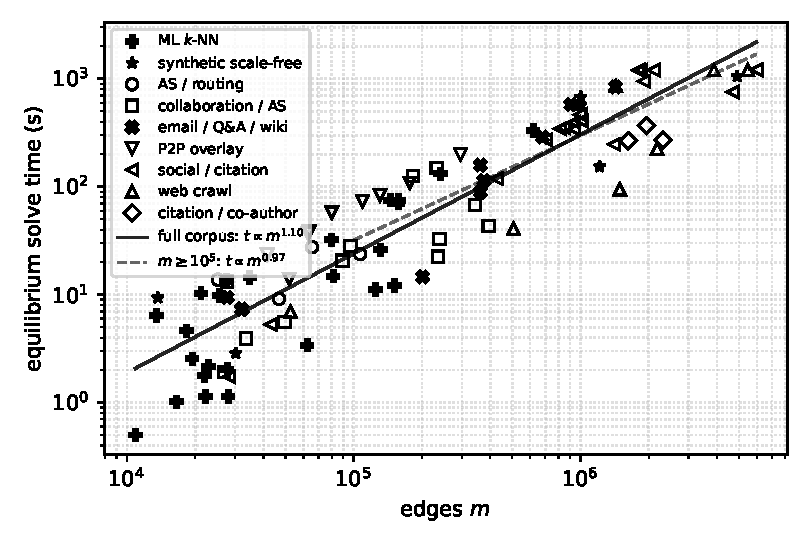
\includegraphics[width=.6\linewidth]{dnlf_corpus.pdf}
\caption{Equilibrium solve time (default LAMG$+$ engine) vs.\ edge count across a topology-diverse corpus of
$53$ irregular SuiteSparse/SNAP graphs (eight families; collaboration and peer-to-peer largest, web and citation
single instances). Wall-clock fits $t\propto m^{0.99}$ over ${\approx}1.45$ decades, with a \emph{bounded}
inner-engine setup count ($[7,27]$)---a descriptive near-linear trend across real graphs of every family, not a
complexity estimate (\cref{sec:results}). Serial, uncontended timing on an Apple M5 Pro.}\label{fig:corpus}\end{figure}

\begin{table}[t]\centering
\caption{Equilibrium solve time (s) on real irregular networks (SuiteSparse/SNAP, largest connected
component): Internet AS graphs and P2P overlays. Near-linear approximate Cholesky vs.\ the fair
frozen-per-level direct baseline; inner-engine \emph{setups} stay size-independent ($14$--$20$ across the corpus).
Single run on one workstation; approximate Cholesky is randomized, so wall-clock and setup counts vary
$\pm$($10$--$30$)\% run to run---the qualitative winner per graph is stable, the third digit is not.
Dash: direct capped at $m>1.5\times10^5$.}
\label{tab:corpus}
\begin{tabular}{lrrrrr}\toprule
graph & $n$ & $m$ & approx.\ Chol. & direct & setups\\\midrule
\texttt{as-735} (AS)         & $6{,}474$  & $25{,}144$  & $35.9$  & $20.5$  & $18$\\
\texttt{p2p-Gnutella08}      & $6{,}299$  & $41{,}552$  & $35.4$  & $53.6$  & $14$\\
\texttt{Oregon-1} (AS)       & $11{,}174$ & $46{,}818$  & $39.7$  & $61.7$  & $20$\\
\texttt{as-caida} (AS)       & $26{,}475$ & $106{,}762$ & $162.0$ & $163.8$ & $18$\\
\texttt{p2p-Gnutella24}      & $26{,}498$ & $130{,}718$ & $262.2$ & $148.0$ & $20$\\
\texttt{ca-HepPh}            & $11{,}204$ & $235{,}238$ & $163.4$ & ---     & $15$\\\bottomrule
\end{tabular}
\end{table}

\begin{table}[t]\centering
\caption{Equilibrium solve time (s) on size-scaled irregular congested networks (random degree-5 graphs), one
clean run on an Apple M5 Pro: the two near-linear engines---LAMG$+$ (default) and approximate Cholesky
(interchangeable)---vs.\ the fair frozen-per-level direct factorization. LAMG$+$ and approximate Cholesky fit the
\emph{same} exponent, $m^{1.11}$, and track within a few percent; direct scales as $m^{1.36}$ and is overtaken
near $m\approx1.5\times10^4$. \emph{OOM}: direct factorization exhausts memory at $m\ge3.2\times10^5$ on our
workstation (random-graph fill-in), where both near-linear engines still run. Approximate Cholesky's randomized
elimination makes it less predictable at the largest size (the $547.7$~s here rose to $856$~s on a second clean
run, vs.\ LAMG$+$'s stable $526$--$533$~s); LAMG$+$ is the default for its cleaner theoretical $O(m)$ guarantee.}
\label{tab:scaling}
\begin{tabular}{rrrrr}\toprule
$n$ & $m$ & LAMG$+$ & approx.\ Cholesky & direct\\\midrule
$1{,}000$  & $9{,}964$   & $4.90$   & $4.93$   & $4.55$\\
$2{,}000$  & $19{,}946$  & $11.01$  & $12.88$  & $10.58$\\
$4{,}000$  & $39{,}952$  & $22.54$  & $20.46$  & $26.81$\\
$8{,}000$  & $79{,}936$  & $52.95$  & $48.24$  & $107.51$\\
$16{,}000$ & $159{,}954$ & $98.65$  & $102.49$ & $160.70$\\
$32{,}000$ & $319{,}952$ & $233.19$ & $229.68$ & \emph{OOM}\\
$64{,}000$ & $639{,}950$ & $526.03$ & $547.68$ & \emph{OOM}\\\bottomrule
\end{tabular}
\end{table}
Bilevel toll design (\cref{alg:design}) therefore inherits a near-linear per-step cost on large irregular
networks, in contrast with the superlinear per-step factorization of the sensitivity-analysis incumbents. On
near-planar road networks the crossover does not occur at practical sizes---nested dissection is near-optimal
there---which is why we frame the advantage on the communication-network regime.

\begin{figure}\centering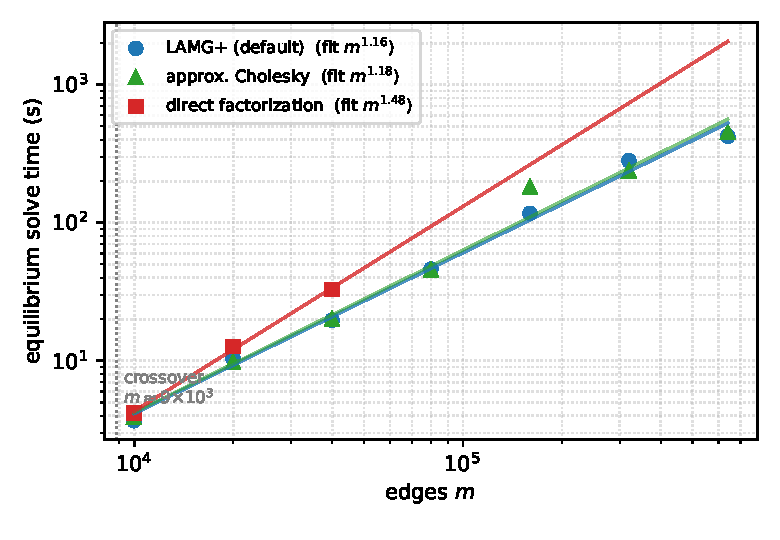
\includegraphics[width=.62\linewidth]{dnlf_scaling.pdf}
\caption{Equilibrium solve time vs.\ edge count on size-scaled irregular congested networks: the two near-linear
engines---LAMG$+$ (default) and approximate Cholesky, both fitting $m^{1.11}$---vs.\ superlinear direct
factorization ($m^{1.36}$), the near-linear engines crossing the direct baseline near
$m\approx1.5\times10^4$.}\label{fig:scaling}\end{figure}

\paragraph{Comparison with differentiable-bilevel (first-order) solvers.}
The learning-based approach to Stackelberg congestion design~\citep{li2022,goyal2023} treats the lower-level
equilibrium as a differentiable layer: it is solved by a first-order scheme (unrolled imitative-logit dynamics;
entropic mirror descent) and differentiated by unrolling or implicit differentiation. Their released code is
toy-scale and does not run on the $10^4$--$10^5$-node irregular graphs here, so we reproduce the defining
component---a first-order inner equilibrium solve---in the same environment and on the same instances. To
isolate the inner solver, both methods minimize the \emph{identical} convex Beckmann energy from the same cold
start; only the inner iteration differs. For the first-order inner we use FISTA (accelerated proximal gradient
with backtracking line search)---a strong, well-tuned member of the first-order family, if anything faster than
plain mirror descent---so the comparison is not a strawman. \Cref{tab:baseline} reports the outcome: our
Newton--multigrid inner reaches relative residual $10^{-9}$ in seconds, whereas FISTA, given a $300$-second
budget on every instance, never reaches the $10^{-6}$ target---it plateaus between $10^{-5}$ on the smallest
graph and $5\times10^{-2}$ on the largest, the residual worsening with size as fewer iterations fit in the
budget. It approaches the same solution (flow within $1.7\%$ on \texttt{as-735}) but never to solve accuracy.
The obstruction is fundamental, not a tuning artifact: heavy congestion makes the
Beckmann Hessian severely ill-conditioned, and an accelerated first-order method still needs
$\Theta(\sqrt{\kappa})$ iterations, so on \texttt{as-735} ($n=6{,}474$) it takes $44{,}499$ iterations to reach
only $1.2\times10^{-2}$. A first-order inner therefore has no fast, size-independent convergence on stiff
equilibria, whereas the Newton--multigrid inner does---which is why these methods are demonstrated only at small
scale, and why replacing their inner solve is the contribution here.

\begin{table}[t]\centering
\caption{Inner-solver head-to-head on the identical convex equilibrium, same cold start. Ours (Newton $+$
approximate Cholesky, loose-intermediate continuation) to relative residual $10^{-9}$; FISTA (accelerated
first-order---the differentiable-bilevel inner) targeting $10^{-6}$ but capped at $300$\,s, which it hits on
every instance, reaching only the residual shown.}
\label{tab:baseline}
\begin{tabular}{lrrrrr}\toprule
instance & $n$ & $m$ & ours (s) & FISTA (s) & FISTA relres\\\midrule
\texttt{synthetic}      & $1{,}000$  & $9{,}964$   & $5.4$  & $300$ & $1.2\times10^{-4}$\\
\texttt{synthetic}      & $2{,}000$  & $19{,}946$  & $12.0$ & $300$ & $2.4\times10^{-5}$\\
\texttt{synthetic}      & $4{,}000$  & $39{,}952$  & $20.6$ & $300$ & $1.0\times10^{-5}$\\
\texttt{p2p-Gnutella08} & $6{,}299$  & $41{,}552$  & $60.4$ & $300$ & $2.4\times10^{-3}$\\
\texttt{Oregon-1}       & $11{,}174$ & $46{,}818$  & $55.5$ & $300$ & $1.6\times10^{-2}$\\
\texttt{as-caida}       & $26{,}475$ & $106{,}762$ & $95.5$ & $300$ & $5.2\times10^{-2}$\\
\end{tabular}
\end{table}

\paragraph{Reproducibility.}
All code, unit tests, and reproduction drivers are available at \url{https://github.com/orenlivne/dnlf}; the
repository regenerates every table and figure in this paper---the crossover (\cref{tab:scaling},
\cref{fig:scaling}), the real-corpus table (\cref{tab:corpus}), the first-order head-to-head
(\cref{tab:baseline}), and the multicommodity tables (\cref{tab:mc,tab:mcdesign,tab:mcreal})---and unit-tests
every algorithm component, including \cref{prop:laplacian,prop:conv,prop:adjoint,prop:mc} and the OD-matrix
loader. All timings reported in this paper were measured on an Apple M5 Pro (18 cores, 48\,GB RAM) under
macOS~26.5. The test networks are the TNTP Sioux Falls and Anaheim instances with their published
OD matrices (shipped with the code) and public Internet AS / P2P-overlay graphs (e.g.\ \texttt{as-caida},
\texttt{Oregon-1}, \texttt{p2p-Gnutella}) from the SuiteSparse/SNAP collection.

\section{Multicommodity logit stochastic user equilibrium and design}\label{sec:mc}
The single-commodity solver of \cref{sec:solver} routes a general balanced demand as one fungible flow.
Realistic congestion pricing is inherently \emph{multicommodity}: each origin--destination (OD) pair routes its
own flow over the shared congested network, and tolls are designed against that coupled equilibrium. We extend
the framework to the multicommodity \emph{logit stochastic user equilibrium} (SUE)~\citep{fisk1980,daganzo1977},
in which route choice has a dispersion $\gamma>0$---a calibrated behavioural parameter, not a numerical
smoothing. The same near-linear machinery carries over: the multicommodity Newton system is a coupled
block-Laplacian that a distribution-matrix block preconditioner solves in a handful of iterations, and the design
adjoint again returns $\nabla_\tau\mathrm{TSTT}$ for all tolls in a single solve.

\paragraph{Formulation.}
With $K$ commodities, per-commodity arc flows $f^k\ge0$, total flow $f_a=\sum_k f^k_a$, and the shared cost
$t_a(f_a)$, the entropic-regularized Beckmann program is
\begin{equation}\label{eq:mcbeck}
  \min_{f^k\ge0}\ \sum_a T_a(f_a)+\gamma\sum_{a,k}f^k_a\bigl(\log f^k_a-1\bigr)
  \quad\text{s.t.}\quad B f^k=d^k,\quad k=1,\dots,K,
\end{equation}
with $T_a'=t_a$. Its stationarity conditions give the \emph{logit assignment}
$f^k_a=\exp\!\bigl((g^k_a-t_a(f_a))/\gamma\bigr)$ with $g^k_a=(B^\top\phi^k)_a$: a per-arc softmax over commodities
whose total $f_a$ solves a monotone scalar fixed point $\log f_a=\mathrm{logsumexp}_k(g^k_a/\gamma)-t_a(f_a)/\gamma$.
As $\gamma\to0$ the model tends to deterministic user equilibrium; we solve at a fixed, calibrated $\gamma$.

\begin{proposition}[multicommodity Newton system: a coupled block Laplacian]\label{prop:mc}
At a logit equilibrium the reduced Newton Jacobian in the stacked potentials $\Phi$ is
\begin{equation}\label{eq:mcjac}
  J=\underbrace{\tfrac1\gamma\,\mathrm{blkdiag}_k\!\bigl(B\,\mathrm{diag}(f^k)\,B^\top\bigr)}_{K\ \text{per-commodity Laplacians}}
   -\tfrac1{\gamma^2}\sum_a c_a\,(f_a f_a^\top)\otimes b_a b_a^\top,
\end{equation}
where $\Phi=[\phi^1;\dots;\phi^K]$, $b_a=Be_a$, $f_a=(f^1_a,\dots,f^K_a)^\top$, and $c_a=t'_a/(1+t'_a f_a/\gamma)$. Each diagonal block is a symmetric weighted graph Laplacian;
the coupling is symmetric positive semidefinite and rank one per arc. For $K=1$, \cref{eq:mcjac} reduces, as
$\gamma\to0$, to the single-commodity active Laplacian $B\,\mathrm{diag}(1/t'_a)\,B^\top$ of \cref{prop:laplacian}.
\end{proposition}
\begin{proof}{\it Proof.}
The equilibrium is $R^k(\Phi)=-Bf^k(\Phi)-d^k=0$. Differentiating the logit map,
$\mathrm{d}f^k_a=(f^k_a/\gamma)(\mathrm{d}g^k_a-t'_a\,\mathrm{d}f_a)$ and $\mathrm{d}f_a=\sum_l\mathrm{d}f^l_a$; solving
the latter gives $\mathrm{d}f_a=(\gamma+t'_af_a)^{-1}\sum_l f^l_a\,\mathrm{d}g^l_a$. Substituting and using
$\mathrm{d}g^k=B^\top\mathrm{d}\phi^k$, $\mathrm{d}R^k=-B\,\mathrm{d}f^k$ yields \cref{eq:mcjac}. Equivalently
$J=\tilde B H^{-1}\tilde B^\top$ with $\tilde B=I_K\otimes B$ and per-arc flow-Hessian
$H_a=t'_a\mathbf1\mathbf1^\top+\gamma\,\mathrm{diag}(1/f^k_a)$; Sherman--Morrison gives
$H_a^{-1}=\tfrac1\gamma\mathrm{diag}(f^k_a)-\tfrac{c_a}{\gamma^2}f_af_a^\top$, and for $K=1$,
$f_a/(\gamma+t'_af_a)\to1/t'_a$ as $\gamma\to0$. \qed
\end{proof}

\paragraph{Near-linear solve.}
We solve \cref{eq:mcbeck} by $\gamma$-continuation damped Newton on $\Phi$, preconditioning \cref{eq:mcjac} by its
block diagonal---one near-linear solve per commodity (approximate Cholesky here, interchangeable with the default
LAMG$+$; on the small, concentrated per-commodity Laplacians the two are equivalent). The rank-one commodity coupling is
exactly Brandt's \emph{distribution matrix}~\citep{brandt1984}: in the mean/deviation basis over commodities it
decouples when the per-commodity Laplacians coincide, so the block preconditioner's rate is governed only by
their spread. Empirically (\cref{tab:mc}) the inner conjugate-gradient count is single digit to low double digit,
grows only logarithmically in $K$, and is independent of graph size $n$ at the operating dispersion
$\gamma\approx0.1$; each Newton step therefore costs $O(K)$ near-linear solves, and the equilibrium solve is
near-linear in the total size $Kn$. Each per-commodity Laplacian carries a small relative conductance floor
($10^{-12}$ of its maximum weight) so it stays connected and the approximate-Cholesky factorization remains
applicable even to a commodity that concentrates on few arcs; a pinned direct solve is retained only as a
fallback for the rare inputs on which the multigrid factorization throws. The count is single digit at and near
equilibrium across all $\gamma$---the regime the warm-started design loop stays in (\cref{tab:mcdesign}); only the
\emph{cold} forward solve at small $\gamma$, far from equilibrium where per-commodity flows concentrate and the
blocks become high-contrast, is expensive, and that regime is entered only as one leaves the logit-SUE model for
its deterministic ($\gamma\to0$) limit. That limit is a \emph{different} model---deterministic multicommodity
user equilibrium, with non-unique commodity flows, for which Frank--Wolfe and related methods are already
effective---not a regime our fixed-$\gamma$ solver must reach: fixed $\gamma$ is a calibrated route-choice
dispersion~\citep{fisk1980,daganzo1977}, a complete behavioural model in its own right, so we solve the logit SUE
at that $\gamma$ and do not pursue $\gamma\to0$. We verified that a coupling-aware distribution-matrix preconditioner
(per-arc coupling inverted by Sherman--Morrison, aggregate-congestion Laplacian on the mean commodity mode, as
\citet{brandt1984} prescribes) converges $\gamma$-boundedly where the reduced-potential version does not, but
does not beat the block diagonal in the operating regime; the block diagonal is retained. Fixed $\gamma$ is thus both the
modelling choice (a calibrated route-choice dispersion) and the regime in which the block preconditioner is well
conditioned.

\paragraph{Design.}
Tolls enter the logit map as a per-arc cost shift $t_a(f_a)+\tau_a$, with flow sensitivity
$\partial f^k_a/\partial\tau_a=-f^k_a c_a$. The same adjoint as \cref{sec:design} returns $\nabla_\tau\mathrm{TSTT}$
for all tolls from a single block-preconditioned solve $J\lambda=\partial_\Phi\mathrm{TSTT}$. The adjoint matches
central finite differences to under $10^{-3}$ (verified by the released unit tests), and on a multicommodity
instance projected-gradient tolling reduces TSTT with the tolls spread across the congested arcs, each
equilibrium re-solve costing single-digit inner iterations---the bilevel iteration inheriting the near-linear
per-step cost. Across a range of synthetic instances (varying $K$, $\gamma$,
network size, and demand; \cref{tab:mcdesign}) the reduction is $1$--$2\%$ and the inner-iteration count stays
single digit. On the two canonical TNTP road networks with their \emph{published} origin--destination matrices
and BPR parameters---Sioux Falls ($n=24$, $m=76$, $K=24$ destination commodities) and Anaheim ($n=416$, $m=914$,
$K=38$)---destination-bundled design reduces the real system travel time by $7.7$--$13.1\%$ (\cref{tab:mcreal}). Both
networks are over-saturated at their full published demand (peak volume/capacity above $2.5$); the inner
iteration count stays bounded and does not grow with size (consistent with the size-independence
established on the synthetic family, \cref{tab:mc}): Anaheim carries $27\times$ the degrees of freedom of Sioux
Falls yet needs \emph{fewer} inner iterations. What sets the count is not size but the per-arc commodity coupling
the block-diagonal preconditioner omits, which is significant only where arcs approach the BPR saturation knee:
tiny, dense Sioux Falls at its over-saturated published demand forces most carrying arcs there, whereas Anaheim
spreads flow so typical arcs stay clear of it. A budget-constrained (sparse-toll) design is a natural extension.

\begin{table}[t]\centering
\caption{Multicommodity logit-SUE inner conjugate-gradient iterations (block-preconditioned) on irregular
networks, $\gamma=0.1$. Left: vs.\ commodities $K$ ($n=1500$), single-OD and spread demands. Right: vs.\ graph
size $n$ ($K=8$, spread). Single-digit to low double digit, $\log K$ growth, $n$-independent.}
\label{tab:mc}
\begin{tabular}{rrr@{\qquad}rr}\toprule
$K$ & single-OD & spread & $n$ (at $K{=}8$) & iters\\\midrule
$2$  & $3$  & $2$  & $1{,}000$ & $6$\\
$4$  & $3$  & $3$  & $2{,}000$ & $6$\\
$8$  & $7$  & $6$  & $4{,}000$ & $7$\\
$12$ & $13$ & $10$ & $8{,}000$ & $3$\\
$16$ & $12$ & $9$  &           &  \\\bottomrule
\end{tabular}
\end{table}

\begin{table}[t]\centering
\caption{Multicommodity toll design across instances (varying commodities $K$, dispersion $\gamma$, network
size $n$, and per-commodity demand ``load''): TSTT reduction, inner conjugate-gradient iterations per
equilibrium re-solve, and the fraction of arcs carrying a \emph{non-negligible} toll ($\tau>10^{-3}$ of the
maximum). The inner count stays single digit throughout.}
\label{tab:mcdesign}
\begin{tabular}{rrrrrrr}\toprule
$n$ & $K$ & $\gamma$ & load & TSTT red.\ & inner it.\ & arcs tolled\\\midrule
$800$     & $4$  & $0.10$ & $3{,}000$ & $1.1\%$ & $3$ & $29\%$\\
$800$     & $8$  & $0.10$ & $3{,}000$ & $1.1\%$ & $4$ & $49\%$\\
$800$     & $16$ & $0.10$ & $3{,}000$ & $1.2\%$ & $7$ & $67\%$\\
$800$     & $8$  & $0.15$ & $3{,}000$ & $1.3\%$ & $3$ & $72\%$\\
$800$     & $8$  & $0.10$ & $6{,}000$ & $1.0\%$ & $6$ & $49\%$\\
$800$     & $8$  & $0.10$ & $3{,}200$ & $1.4\%$ & $6$ & $45\%$\\
$1{,}200$ & $8$  & $0.10$ & $3{,}600$ & $1.4\%$ & $6$ & $44\%$\\
$1{,}600$ & $8$  & $0.10$ & $3{,}600$ & $1.2\%$ & $6$ & $43\%$\\\bottomrule
\end{tabular}
\end{table}

\begin{table}[t]\centering
\caption{Real-network validation: destination-bundled logit-SUE toll design on the two canonical TNTP road
networks with their \emph{published} OD matrices and BPR parameters (one commodity per destination zone). Both
are over-saturated at full demand (peak volume/capacity $>2.5$). Tolls spread across $53$--$74\%$ of arcs. The
inner conjugate-gradient count at the final equilibrium solve is bounded ($12$--$38$); it is set by proximity
to the BPR saturation knee (\cref{sec:mc}), not by network size---Anaheim has $27\times$ the degrees of freedom
of Sioux Falls yet needs fewer iterations.}
\label{tab:mcreal}
\begin{tabular}{lrrrrrr}\toprule
network & $n$ & $m$ & $K$ & $\gamma$ & TSTT red.\ & inner it.\\\midrule
Sioux Falls & $24$  & $76$  & $24$ & $2$ & $9.4\%$  & $38$\\
Sioux Falls & $24$  & $76$  & $24$ & $5$ & $13.1\%$ & $30$\\
Anaheim     & $416$ & $914$ & $38$ & $2$ & $12.2\%$ & $16$\\
Anaheim     & $416$ & $914$ & $38$ & $5$ & $\phantom{0}7.7\%$  & $12$\\\bottomrule
\end{tabular}
\end{table}

\section{Related work}\label{sec:related}
\paragraph{Bilevel network design and sensitivity.}
CNDP and second-best tolling are bilevel/MPEC problems, nonconvex and \emph{NP}-hard~\citep{gairing2017,hoefer2008};
surveys~\citep{farahani2013} catalog SAB descent, MPEC, and metaheuristic methods. Equilibrium sensitivity
originates with \citet{tobinfriesz1988} and was sharpened by Qiu and Magnanti and by Patriksson
and co-authors~\citep{jp2007}, who observed that the sensitivity problem is itself a linearized equilibrium solve.
Our adjoint \cref{eq:adjoint} is precisely that observation; the novelty here is not the $k$-independent gradient
but the \emph{near-linear} operator that computes it and the forward solve. The same bilevel problem is studied
in algorithmic game theory as optimal tolling and Stackelberg routing to reduce the price of anarchy of a
congestion game~\citep{roughgarden2002,swamy2012,korilis1997,cole2003}, and in communication networks as competitive /
selfish routing~\citep{orda1993,larroca2013}; that literature focuses on existence, bounds, and mechanism design
rather than on a scalable solver for the induced equilibrium, which is our concern. Recent differentiable-bilevel
methods
\citep{li2022,goyal2023} break the cold-resolve-per-step pattern with warm-started, truncated first-order inner
loops and unrolled/implicit differentiation, but use no multigrid and are demonstrated only at Sioux
Falls--Chicago-Sketch scale. Their defining component is a first-order inner equilibrium solve; we compare
head-to-head against a strong instance of it (FISTA on the same convex Beckmann energy) in \cref{sec:results}.

\paragraph{Near-linear Laplacian solvers and nonlinear flow.}
Nearly-linear-time solvers for symmetric diagonally dominant systems~\citep{kyngsachdeva2016,lamgplus} underpin
web-scale spectral graph computation but have not, to our knowledge, been used as the inner solve of a bilevel
traffic-design loop. The nonlinear Laplacian flow framework~\citep{nlf} unifies max-flow, congestion, and
min-delay routing as one monotone edge-law equation and supplies the chord-Newton machinery we build on;
the present work extends it from the undirected relaxation to the directed (rectified) equilibrium and to the
design (adjoint) problem.

\section{Conclusions, limitations, and open problems}\label{sec:conclusion}
We showed that the directed user equilibrium with separable costs is a nonlinear Laplacian flow whose Jacobian
is a symmetric active-subgraph Laplacian, so a smoothing homotopy reduces the forward solve and the adjoint
design gradient to a short sequence of near-linear Laplacian solves with a graph-size-independent number of
multigrid setups; bilevel toll design inherits this near-linear per-step cost, in place of the cubic
factorization of sensitivity-analysis methods.

We are explicit about what this paper does \emph{not} yet establish. (i) \textbf{Multicommodity scope.}
\Cref{sec:mc} solves and designs the multicommodity logit SUE at fixed calibrated $\gamma$; we do not pursue the
$\gamma\to0$ deterministic limit, a distinct model (non-unique per-commodity flows) already served by
Frank--Wolfe. (ii) \textbf{Corpus scaling.} A still-larger corpus (thousands of graphs) would tighten the
descriptive $m^{0.99}$ fit of \cref{fig:corpus}. (iii) \textbf{One hierarchy across design steps.} Each exact
solve rebuilds once per $\delta$-level because crossing an active-set boundary raises a near-null-space mode;
capturing that mode by deflation or recombination would make one hierarchy valid across all design steps and cut
the setups to $\mathcal{O}(1)$ \emph{total}---the main open algorithmic problem. (iv) \textbf{Planarity.} The
advantage is on non-planar, poorly-separable topologies; on near-planar road networks nested dissection is
already near-optimal (\cref{sec:intro}). (v) \textbf{Saturating laws and folds.} A capacity-saturating
(min-delay) law reintroduces a turning-point fold; design through the fold, via the continuation/deflation
of~\citet{nlf}, is future work.

\ACKNOWLEDGMENT{This work builds on the NLF and LAMG$+$ solvers; the author thanks the developers of the
approximate-Cholesky implementation it uses.}

\begin{thebibliography}{}
\bibitem[Tobin and Friesz(1988)]{tobinfriesz1988} R.~L.~Tobin and T.~L.~Friesz, \emph{Sensitivity analysis for equilibrium network flow},
Transportation Science, 22 (1988), pp.~242--250.
\bibitem[Josefsson and Patriksson(2007)]{jp2007} M.~Josefsson and M.~Patriksson, \emph{Sensitivity analysis of separable traffic equilibria with
application to bilevel optimization in network design}, Transportation Research Part B, 41 (2007), pp.~4--31.
\bibitem[Chiou(2005)]{chiou2005} S.-W.~Chiou, \emph{Bilevel programming for the continuous transport network design problem},
Transportation Research Part B, 39 (2005), pp.~361--383.
\bibitem[Gairing et al.(2017)]{gairing2017} M.~Gairing, T.~Harks, and M.~Klimm, \emph{Complexity and approximation of the continuous
network design problem}, SIAM Journal on Optimization, 27 (2017), pp.~1554--1582.
\bibitem[Hoefer et al.(2008)]{hoefer2008} M.~Hoefer, L.~Olbrich, and A.~Skopalik, \emph{Taxing subnetworks}, in Proc.\ WINE, 2008,
pp.~286--294.
\bibitem[Farahani et al.(2013)]{farahani2013} R.~Z.~Farahani, E.~Miandoabchi, W.~Y.~Szeto, and H.~Rashidi, \emph{A review of urban
transportation network design problems}, European Journal of Operational Research, 229 (2013), pp.~281--302.
\bibitem[Bar-Gera(2002)]{bargera2002} H.~Bar-Gera, \emph{Origin-based algorithm for the traffic assignment problem},
Transportation Science, 36 (2002), pp.~398--417.
\bibitem[Dial(2006)]{dial2006} R.~B.~Dial, \emph{A path-based user-equilibrium traffic assignment algorithm that obviates
path storage and enumeration}, Transportation Research Part B, 40 (2006), pp.~917--936.
\bibitem[Li et al.(2022)]{li2022} P.~Li et al., \emph{Differentiable bilevel programming for Stackelberg congestion games},
arXiv:2209.07618, 2022.
\bibitem[Goyal and Lamperski(2023)]{goyal2023} A.~Goyal and A.~Lamperski, \emph{An algorithm for bilevel optimization with traffic
equilibrium constraints}, arXiv:2306.14235, 2023.
\bibitem[Kyng and Sachdeva(2016)]{kyngsachdeva2016} R.~Kyng and S.~Sachdeva, \emph{Approximate Gaussian elimination for Laplacians---fast,
sparse, and simple}, in Proc.\ FOCS, 2016, pp.~573--582.
\bibitem[Livne(2026a)]{lamgplus} O.~E.~Livne, \emph{LAMG$+$: a robust lean algebraic multigrid solver for graph Laplacians},
arXiv:2606.24791; accepted, SIAM Journal on Scientific Computing.
\bibitem[Livne(2026b)]{nlf} O.~E.~Livne, \emph{NLF: a resistor-network framework and linear-time solver for convex network-flow
equilibria}, SIAM Journal on Scientific Computing (under review), 2026.
\bibitem[Fisk(1980)]{fisk1980} C.~Fisk, \emph{Some developments in equilibrium traffic assignment}, Transportation Research
Part B, 14 (1980), pp.~243--255.
\bibitem[Daganzo and Sheffi(1977)]{daganzo1977} C.~F.~Daganzo and Y.~Sheffi, \emph{On stochastic models of traffic assignment},
Transportation Science, 11 (1977), pp.~253--274.
\bibitem[Brandt(1984)]{brandt1984} A.~Brandt, \emph{Multigrid techniques: 1984 guide with applications to fluid dynamics},
GMD-Studien Nr.~85, Gesellschaft f\"ur Mathematik und Datenverarbeitung, 1984 (distributive/distribution-matrix
relaxation, \S3.4).
\bibitem[Amos and Kolter(2017)]{amos2017} B.~Amos and J.~Z.~Kolter, \emph{OptNet: differentiable optimization as a layer in neural
networks}, in Proc.\ ICML, 2017, pp.~136--145.
\bibitem[Blondel et al.(2022)]{blondel2022} M.~Blondel et al., \emph{Efficient and modular implicit differentiation}, in Proc.\
NeurIPS, 2022.
\bibitem[Rosenthal(1973)]{rosenthal1973} R.~W.~Rosenthal, \emph{A class of games possessing pure-strategy Nash equilibria},
International Journal of Game Theory, 2 (1973), pp.~65--67.
\bibitem[Roughgarden and Tardos(2002)]{roughgarden2002} T.~Roughgarden and \'E.~Tardos, \emph{How bad is selfish routing?}, Journal of the
ACM, 49 (2002), pp.~236--259.
\bibitem[Swamy(2012)]{swamy2012} C.~Swamy, \emph{The effectiveness of Stackelberg strategies and tolls for network congestion
games}, ACM Transactions on Algorithms, 8 (2012), art.~36.
\bibitem[Korilis et al.(1997)]{korilis1997} Y.~A.~Korilis, A.~A.~Lazar, and A.~Orda, \emph{Achieving network optima using Stackelberg
routing strategies}, IEEE/ACM Transactions on Networking, 5 (1997), pp.~161--173.
\bibitem[Orda et al.(1993)]{orda1993} A.~Orda, R.~Rom, and N.~Shimkin, \emph{Competitive routing in multiuser communication
networks}, IEEE/ACM Transactions on Networking, 1 (1993), pp.~510--521.
\bibitem[Larroca and Rougier(2013)]{larroca2013} F.~Larroca and J.-L.~Rougier, \emph{Minimum-delay load-balancing through non-parametric
regression and traffic-engineering}, Computer Networks, 57 (2013), pp.~2716--2728.
\bibitem[Qiu et al.(2003)]{qiu2003} L.~Qiu, Y.~R.~Yang, Y.~Zhang, and S.~Shenker, \emph{On selfish routing in Internet-like
environments}, in Proc.\ ACM SIGCOMM, 2003, pp.~151--162.
\bibitem[Faloutsos et al.(1999)]{faloutsos1999} M.~Faloutsos, P.~Faloutsos, and C.~Faloutsos, \emph{On power-law relationships of the
Internet topology}, in Proc.\ ACM SIGCOMM, 1999, pp.~251--262.
\bibitem[Fortz and Thorup(2000)]{fortz2000} B.~Fortz and M.~Thorup, \emph{Internet traffic engineering by optimizing OSPF weights}, in
Proc.\ IEEE INFOCOM, 2000, pp.~519--528.
\bibitem[Cole et al.(2003)]{cole2003} R.~Cole, Y.~Dodis, and T.~Roughgarden, \emph{Pricing network edges for heterogeneous selfish
users}, in Proc.\ ACM STOC, 2003, pp.~521--530.
\bibitem[Leskovec et al.(2007)]{leskovec2007} J.~Leskovec, J.~Kleinberg, and C.~Faloutsos, \emph{Graph evolution: densification and
shrinking diameters}, ACM Trans.\ Knowledge Discovery from Data, 1 (2007), art.~2.
\end{thebibliography}
\end{document}
